\documentclass[]{scrbook}
\usepackage{lmodern}
\usepackage{amssymb,amsmath}
\usepackage{ifxetex,ifluatex}
\usepackage{fixltx2e} % provides \textsubscript
\ifnum 0\ifxetex 1\fi\ifluatex 1\fi=0 % if pdftex
  \usepackage[T1]{fontenc}
  \usepackage[utf8]{inputenc}
\else % if luatex or xelatex
  \ifxetex
    \usepackage{mathspec}
  \else
    \usepackage{fontspec}
  \fi
  \defaultfontfeatures{Ligatures=TeX,Scale=MatchLowercase}
\fi
% use upquote if available, for straight quotes in verbatim environments
\IfFileExists{upquote.sty}{\usepackage{upquote}}{}
% use microtype if available
\IfFileExists{microtype.sty}{%
\usepackage[]{microtype}
\UseMicrotypeSet[protrusion]{basicmath} % disable protrusion for tt fonts
}{}
\PassOptionsToPackage{hyphens}{url} % url is loaded by hyperref
\usepackage[unicode=true]{hyperref}
\hypersetup{
            pdftitle={Penn State Integrated Hydrologic Model(PIHM)},
            pdfauthor={Lele Shu (lele.shu@gmail.com)},
            pdfborder={0 0 0},
            breaklinks=true}
\urlstyle{same}  % don't use monospace font for urls
\usepackage{natbib}
\bibliographystyle{apalike}
\usepackage{color}
\usepackage{fancyvrb}
\newcommand{\VerbBar}{|}
\newcommand{\VERB}{\Verb[commandchars=\\\{\}]}
\DefineVerbatimEnvironment{Highlighting}{Verbatim}{commandchars=\\\{\}}
% Add ',fontsize=\small' for more characters per line
\usepackage{framed}
\definecolor{shadecolor}{RGB}{248,248,248}
\newenvironment{Shaded}{\begin{snugshade}}{\end{snugshade}}
\newcommand{\KeywordTok}[1]{\textcolor[rgb]{0.13,0.29,0.53}{\textbf{#1}}}
\newcommand{\DataTypeTok}[1]{\textcolor[rgb]{0.13,0.29,0.53}{#1}}
\newcommand{\DecValTok}[1]{\textcolor[rgb]{0.00,0.00,0.81}{#1}}
\newcommand{\BaseNTok}[1]{\textcolor[rgb]{0.00,0.00,0.81}{#1}}
\newcommand{\FloatTok}[1]{\textcolor[rgb]{0.00,0.00,0.81}{#1}}
\newcommand{\ConstantTok}[1]{\textcolor[rgb]{0.00,0.00,0.00}{#1}}
\newcommand{\CharTok}[1]{\textcolor[rgb]{0.31,0.60,0.02}{#1}}
\newcommand{\SpecialCharTok}[1]{\textcolor[rgb]{0.00,0.00,0.00}{#1}}
\newcommand{\StringTok}[1]{\textcolor[rgb]{0.31,0.60,0.02}{#1}}
\newcommand{\VerbatimStringTok}[1]{\textcolor[rgb]{0.31,0.60,0.02}{#1}}
\newcommand{\SpecialStringTok}[1]{\textcolor[rgb]{0.31,0.60,0.02}{#1}}
\newcommand{\ImportTok}[1]{#1}
\newcommand{\CommentTok}[1]{\textcolor[rgb]{0.56,0.35,0.01}{\textit{#1}}}
\newcommand{\DocumentationTok}[1]{\textcolor[rgb]{0.56,0.35,0.01}{\textbf{\textit{#1}}}}
\newcommand{\AnnotationTok}[1]{\textcolor[rgb]{0.56,0.35,0.01}{\textbf{\textit{#1}}}}
\newcommand{\CommentVarTok}[1]{\textcolor[rgb]{0.56,0.35,0.01}{\textbf{\textit{#1}}}}
\newcommand{\OtherTok}[1]{\textcolor[rgb]{0.56,0.35,0.01}{#1}}
\newcommand{\FunctionTok}[1]{\textcolor[rgb]{0.00,0.00,0.00}{#1}}
\newcommand{\VariableTok}[1]{\textcolor[rgb]{0.00,0.00,0.00}{#1}}
\newcommand{\ControlFlowTok}[1]{\textcolor[rgb]{0.13,0.29,0.53}{\textbf{#1}}}
\newcommand{\OperatorTok}[1]{\textcolor[rgb]{0.81,0.36,0.00}{\textbf{#1}}}
\newcommand{\BuiltInTok}[1]{#1}
\newcommand{\ExtensionTok}[1]{#1}
\newcommand{\PreprocessorTok}[1]{\textcolor[rgb]{0.56,0.35,0.01}{\textit{#1}}}
\newcommand{\AttributeTok}[1]{\textcolor[rgb]{0.77,0.63,0.00}{#1}}
\newcommand{\RegionMarkerTok}[1]{#1}
\newcommand{\InformationTok}[1]{\textcolor[rgb]{0.56,0.35,0.01}{\textbf{\textit{#1}}}}
\newcommand{\WarningTok}[1]{\textcolor[rgb]{0.56,0.35,0.01}{\textbf{\textit{#1}}}}
\newcommand{\AlertTok}[1]{\textcolor[rgb]{0.94,0.16,0.16}{#1}}
\newcommand{\ErrorTok}[1]{\textcolor[rgb]{0.64,0.00,0.00}{\textbf{#1}}}
\newcommand{\NormalTok}[1]{#1}
\usepackage{longtable,booktabs}
% Fix footnotes in tables (requires footnote package)
\IfFileExists{footnote.sty}{\usepackage{footnote}\makesavenoteenv{long table}}{}
\usepackage{graphicx,grffile}
\makeatletter
\def\maxwidth{\ifdim\Gin@nat@width>\linewidth\linewidth\else\Gin@nat@width\fi}
\def\maxheight{\ifdim\Gin@nat@height>\textheight\textheight\else\Gin@nat@height\fi}
\makeatother
% Scale images if necessary, so that they will not overflow the page
% margins by default, and it is still possible to overwrite the defaults
% using explicit options in \includegraphics[width, height, ...]{}
\setkeys{Gin}{width=\maxwidth,height=\maxheight,keepaspectratio}
\IfFileExists{parskip.sty}{%
\usepackage{parskip}
}{% else
\setlength{\parindent}{0pt}
\setlength{\parskip}{6pt plus 2pt minus 1pt}
}
\setlength{\emergencystretch}{3em}  % prevent overfull lines
\providecommand{\tightlist}{%
  \setlength{\itemsep}{0pt}\setlength{\parskip}{0pt}}
\setcounter{secnumdepth}{5}
% Redefines (sub)paragraphs to behave more like sections
\ifx\paragraph\undefined\else
\let\oldparagraph\paragraph
\renewcommand{\paragraph}[1]{\oldparagraph{#1}\mbox{}}
\fi
\ifx\subparagraph\undefined\else
\let\oldsubparagraph\subparagraph
\renewcommand{\subparagraph}[1]{\oldsubparagraph{#1}\mbox{}}
\fi

% set default figure placement to htbp
\makeatletter
\def\fps@figure{htbp}
\makeatother

\usepackage{booktabs}

\title{Penn State Integrated Hydrologic Model(PIHM)}
\providecommand{\subtitle}[1]{}
\subtitle{Theoretical Documentation}
\author{Lele Shu
(\href{mailto:lele.shu@gmail.com}{\nolinkurl{lele.shu@gmail.com}})}
\date{2019-05-03}

\begin{document}
\maketitle

{
\setcounter{tocdepth}{1}
\tableofcontents
}
\chapter{Introduction}\label{intro}

\textbf{PIHM} The Penn State Integrated Hydrologic Model (PIHM) is a
multiprocess, multi-scale hydrologic model where the major hydrological
processes are fully coupled using the semi-discrete Finite Volume
Method.

\textbf{PIHMGIS} The model itself is ``tightly-coupled'' with PIHMgis,
an open-source Geographical Information System designed for PIHM. The
PIHMgis provides the access to the digital data sets (terrain, forcing
and parameters) and tools necessary to drive the model, as well as a
collection of GIS-based pre- and post-processing tools.

Collectively the system is referred to as the Penn State Integrated
Hydrologic Modeling System (PIHMS).

The PIHM is an open source software, freely available for download at
\href{www.pihm.psu.edu}{PIHM website} or
\href{https://github.com/shulele/PIHM++}{Github Page} along with
installation and user guides.

\section{Why PIHM?}\label{why-pihm}

It is our intention to begin a debate on the role of \emph{Community
Models} in the hydrologic sciences. Our research is a response to recent
trends in US funding for \emph{Observatory Science} that have emerged at
NSF over the last few years, namely, the NSF-funded \textbf{CUAHSI}
program (Consortium of Universities for Advanicing Hydrologic Sciences).

PIHM represents our strategy for the synthesis of \emph{multi-state},
\emph{multiscale} distributed hydrologic models using the integral
representation of the underlying physical process equations and state
variables.

Our interest is in devising a concise representation of watershed and/or
river basin hydrodynamics, which allows interactions among major
physical processes operating simultaneously, but with the flexibility to
add or eliminate states/processes/constitutive relations depending on
the objective of the numerical experiment or purpose of the scientific
or operational application.

To satisfy the objectives, the PIHM

\begin{itemize}
\tightlist
\item
  is distributed hydrologic model, based on the semi-discrete
  \textbf{Finite-Volume Method (FVM)} in which domain discretization is
  an unstructured triangular irregular network (e.g.~Delaunay triangles)
  generated with constraints (geometric, and parametric). A local
  prismatic control volume is formed by vertical projection of the
  Delauney triangles forming each layer of the model. Given a set of
  constraints (e.g.~river network support, watershed boundary, altitude
  zones, ecological regions, hydraulic properties, climate zones, etc),
  an ``optimal'' mesh is generated. River volume elements are also
  prismatic, with trapezoidal or rectangular cross-section, and are
  generated along or cross edges of Delauney triangles. The local
  control volume contains all equations to be solved and is referred to
  as the model kernel.
\item
  is physically-based model, in which all equations used is descibing
  the physics of the hydrological processes which control the catchment.
  The physical model is ablr to predict the water in ungage water
  system, to estimate the sediment, pullutants and vegetation etc, such
  that it is practical to be coupled with biochemistry, geomorphology,
  limnology and other water-related research. The global ODE system is
  assembled by combining all local ODE systems throughout the domain and
  then solved by a state-of-the-art parallel ODE solver known as CVODE
  developed at the Lawrence- Livermore National Laboratory.
\item
  is fully-couple hydrologic model, where the state and flux variables
  in the hydrologic system are solved within same time step and conserve
  the mass. The fluxes are infiltration, overland flow, groundwater
  recharge, lateral groundwater flow, exchange of river and
  soil/groundwater and river discharge.
\item
  is adaptable temporal and spatial resolution. The spatial resolution
  of model varies from meters to kilometers based requirement of
  modeling and computing resources. Internal time step of iteration step
  are adjustable; it is able to export the status of catchment in less 1
  sencond to days. Also the time interval for exporting results is
  configured flexiblly. The flexible spatial and temporal resolution is
  rather valueable for community model coupling.
\item
  is open source model, anyone can access the source code, use and
  submit their improvement.
\item
  is long-term yield and single-event flood model.
\end{itemize}

An important partnership and motivation for this work was the Project
Leaders participation in two community-science research activites over
the last few years: The University of Arizona-led Science and Technology
Center (SAHRA: Sustainability of Water Resources in Semi- Arid Regions),
and the Chesapeake Community Modeling Project (CCMP). Each of these
research programs has been essential to supporting the concept of
\textbf{Community Models} for environmental prediction and helping to
make it happen.

\section{History of PIHM system}\label{history-of-pihm-system}

\begin{itemize}
\tightlist
\item
  2005 PIHM v1.0
\end{itemize}

Dr Yizhong Qu developed and verified the first version of PIHM in
2001-2005 during his PhD in Pennsylvania State Unversity, following the
blueprint of Freeze and Harlan (1969). This version of PIHM is the soul
of the PIHM model.

\begin{itemize}
\tightlist
\item
  2009 PIHMgis
\end{itemize}

Dr.~Gopal Bhartt developed the PIHMgis with support of C++, Qt GUI
library, TRIANGLE library and QGIS developing kit. The developmemnt of
PIHMgis make the learning curve of PIHM moderate and benefits the
developing, modeling and coupling.

\begin{itemize}
\tightlist
\item
  2015 MM-PIHM
\end{itemize}

Dr.~Yuninh Shi led and developed the MM-PIHM (Multi-Module PIHM), which
embeded the all modules from PIHM family, such as RT-PIHM, LE-PIHM,
flux-PIHM, BGC-PIHM etc. together. The sophysiticated design and
coupling of the MM-PIHM is the summit of the PIHM as a \emph{Community
Model} that combined all water-related module together.

\begin{itemize}
\tightlist
\item
  2019 PIHM++
\end{itemize}

Based on the accumulated contribution of PIHM modeling and coupling with
related researches, it is neccessary to solve the known bugs and
limitation, improve the performance of model with parrellel methods, and
adopt new update from SUNDIALS solver and programming strategy. \#\#
Steps of PIHM modeling

\subsection{Essential Terrestrial
Variables?}\label{essential-terrestrial-variables}

\begin{itemize}
\tightlist
\item
  Atmospheric Forcing (precipitation, snow cover, wind, relative
  humidity, temperature, net radiation, albedo, photosynthestic
  atmospheric radiation, leaf area index)
\item
  Digital elevation models
\item
  River/Stream Discharge
\item
  Soil (class, hydrologic properties)
\item
  Groundwater (levels, extent, hydro-geologic properties)
\item
  Lake/Reservoir (levels, extent)
\item
  Land Cover/Use (biomass, human infrastructure, demography, ecosystem
  disturbance)
\item
  Water Use
\end{itemize}

Most data reside on federal servers \ldots{}.many petabytes

\subsection{A-Priori Data Sources}\label{a-priori-data-sources}

\begin{longtable}[]{@{}ccc@{}}
\toprule
\begin{minipage}[b]{0.18\columnwidth}\centering\strut
Feature/Time-Series\strut
\end{minipage} & \begin{minipage}[b]{0.24\columnwidth}\centering\strut
Property\strut
\end{minipage} & \begin{minipage}[b]{0.43\columnwidth}\centering\strut
Source\strut
\end{minipage}\tabularnewline
\midrule
\endhead
\begin{minipage}[t]{0.18\columnwidth}\centering\strut
Soil\strut
\end{minipage} & \begin{minipage}[t]{0.24\columnwidth}\centering\strut
Porosity; Sand, Silt, Clay Fractions; Bulk Density\strut
\end{minipage} & \begin{minipage}[t]{0.43\columnwidth}\centering\strut
CONUS, SSURGO and STATSGO\strut
\end{minipage}\tabularnewline
\begin{minipage}[t]{0.18\columnwidth}\centering\strut
Geology\strut
\end{minipage} & \begin{minipage}[t]{0.24\columnwidth}\centering\strut
Bed Rock Depth; Horizontal and Vertical Hydraulic Conductivity\strut
\end{minipage} & \begin{minipage}[t]{0.43\columnwidth}\centering\strut
\url{http://www.dcnr.state.pa.us/topogeo/},
\url{http://www.lias.psu.edu/emsl/guides/X.html}\strut
\end{minipage}\tabularnewline
\begin{minipage}[t]{0.18\columnwidth}\centering\strut
Land Cover\strut
\end{minipage} & \begin{minipage}[t]{0.24\columnwidth}\centering\strut
LAI\strut
\end{minipage} & \begin{minipage}[t]{0.43\columnwidth}\centering\strut
\href{http://glcf.umiacs.umd.edu/data/landcover/data.shtml}{UMC},
\href{http://ldas.gsfc.nasa.gov/LDAS8th/MAPPED.VEG/LDASmapveg.shtml}{LDASmapveg};\strut
\end{minipage}\tabularnewline
\begin{minipage}[t]{0.18\columnwidth}\centering\strut
Land Cover\strut
\end{minipage} & \begin{minipage}[t]{0.24\columnwidth}\centering\strut
Manning's Roughness;\strut
\end{minipage} & \begin{minipage}[t]{0.43\columnwidth}\centering\strut
Hernandez et. al., 2000\strut
\end{minipage}\tabularnewline
\begin{minipage}[t]{0.18\columnwidth}\centering\strut
River\strut
\end{minipage} & \begin{minipage}[t]{0.24\columnwidth}\centering\strut
Manning's Roughness;\strut
\end{minipage} & \begin{minipage}[t]{0.43\columnwidth}\centering\strut
Dingman (2002)\strut
\end{minipage}\tabularnewline
\begin{minipage}[t]{0.18\columnwidth}\centering\strut
River\strut
\end{minipage} & \begin{minipage}[t]{0.24\columnwidth}\centering\strut
Coefficient of Discharge\strut
\end{minipage} & \begin{minipage}[t]{0.43\columnwidth}\centering\strut
ModHms Manual (Panday and Huyakorn, 2004)\strut
\end{minipage}\tabularnewline
\begin{minipage}[t]{0.18\columnwidth}\centering\strut
River\strut
\end{minipage} & \begin{minipage}[t]{0.24\columnwidth}\centering\strut
Shape and Dimensions;\strut
\end{minipage} & \begin{minipage}[t]{0.43\columnwidth}\centering\strut
Derived from regression using depth, width and discharge data from
\href{http://nwis.waterdata.usgs.gov/usa/nwis/measurements}{USGS
data}\strut
\end{minipage}\tabularnewline
\begin{minipage}[t]{0.18\columnwidth}\centering\strut
River\strut
\end{minipage} & \begin{minipage}[t]{0.24\columnwidth}\centering\strut
Topology: Nodes, Neighboring Elements;\strut
\end{minipage} & \begin{minipage}[t]{0.43\columnwidth}\centering\strut
Derived using PIHMgis (Bhatt et. al., 2008)\strut
\end{minipage}\tabularnewline
\begin{minipage}[t]{0.18\columnwidth}\centering\strut
Forcing\strut
\end{minipage} & \begin{minipage}[t]{0.24\columnwidth}\centering\strut
Prec, Temp. RH, Wind, Rad.\strut
\end{minipage} & \begin{minipage}[t]{0.43\columnwidth}\centering\strut
National Land Data Assimilation System : NLDAS-2\strut
\end{minipage}\tabularnewline
\begin{minipage}[t]{0.18\columnwidth}\centering\strut
Topography\strut
\end{minipage} & \begin{minipage}[t]{0.24\columnwidth}\centering\strut
DEM\strut
\end{minipage} & \begin{minipage}[t]{0.43\columnwidth}\centering\strut
\url{http://seamless.usgs.gov/}\strut
\end{minipage}\tabularnewline
\begin{minipage}[t]{0.18\columnwidth}\centering\strut
Streamflow\strut
\end{minipage} & \begin{minipage}[t]{0.24\columnwidth}\centering\strut
\strut
\end{minipage} & \begin{minipage}[t]{0.43\columnwidth}\centering\strut
\url{http://nwis.waterdata.usgs.gov/nwis/sw}\strut
\end{minipage}\tabularnewline
\begin{minipage}[t]{0.18\columnwidth}\centering\strut
Groundwater\strut
\end{minipage} & \begin{minipage}[t]{0.24\columnwidth}\centering\strut
\strut
\end{minipage} & \begin{minipage}[t]{0.43\columnwidth}\centering\strut
\url{http://nwis.waterdata.usgs.gov/nwis/gw}\strut
\end{minipage}\tabularnewline
\bottomrule
\end{longtable}

\section{Steps}\label{steps}

\begin{figure}
\centering
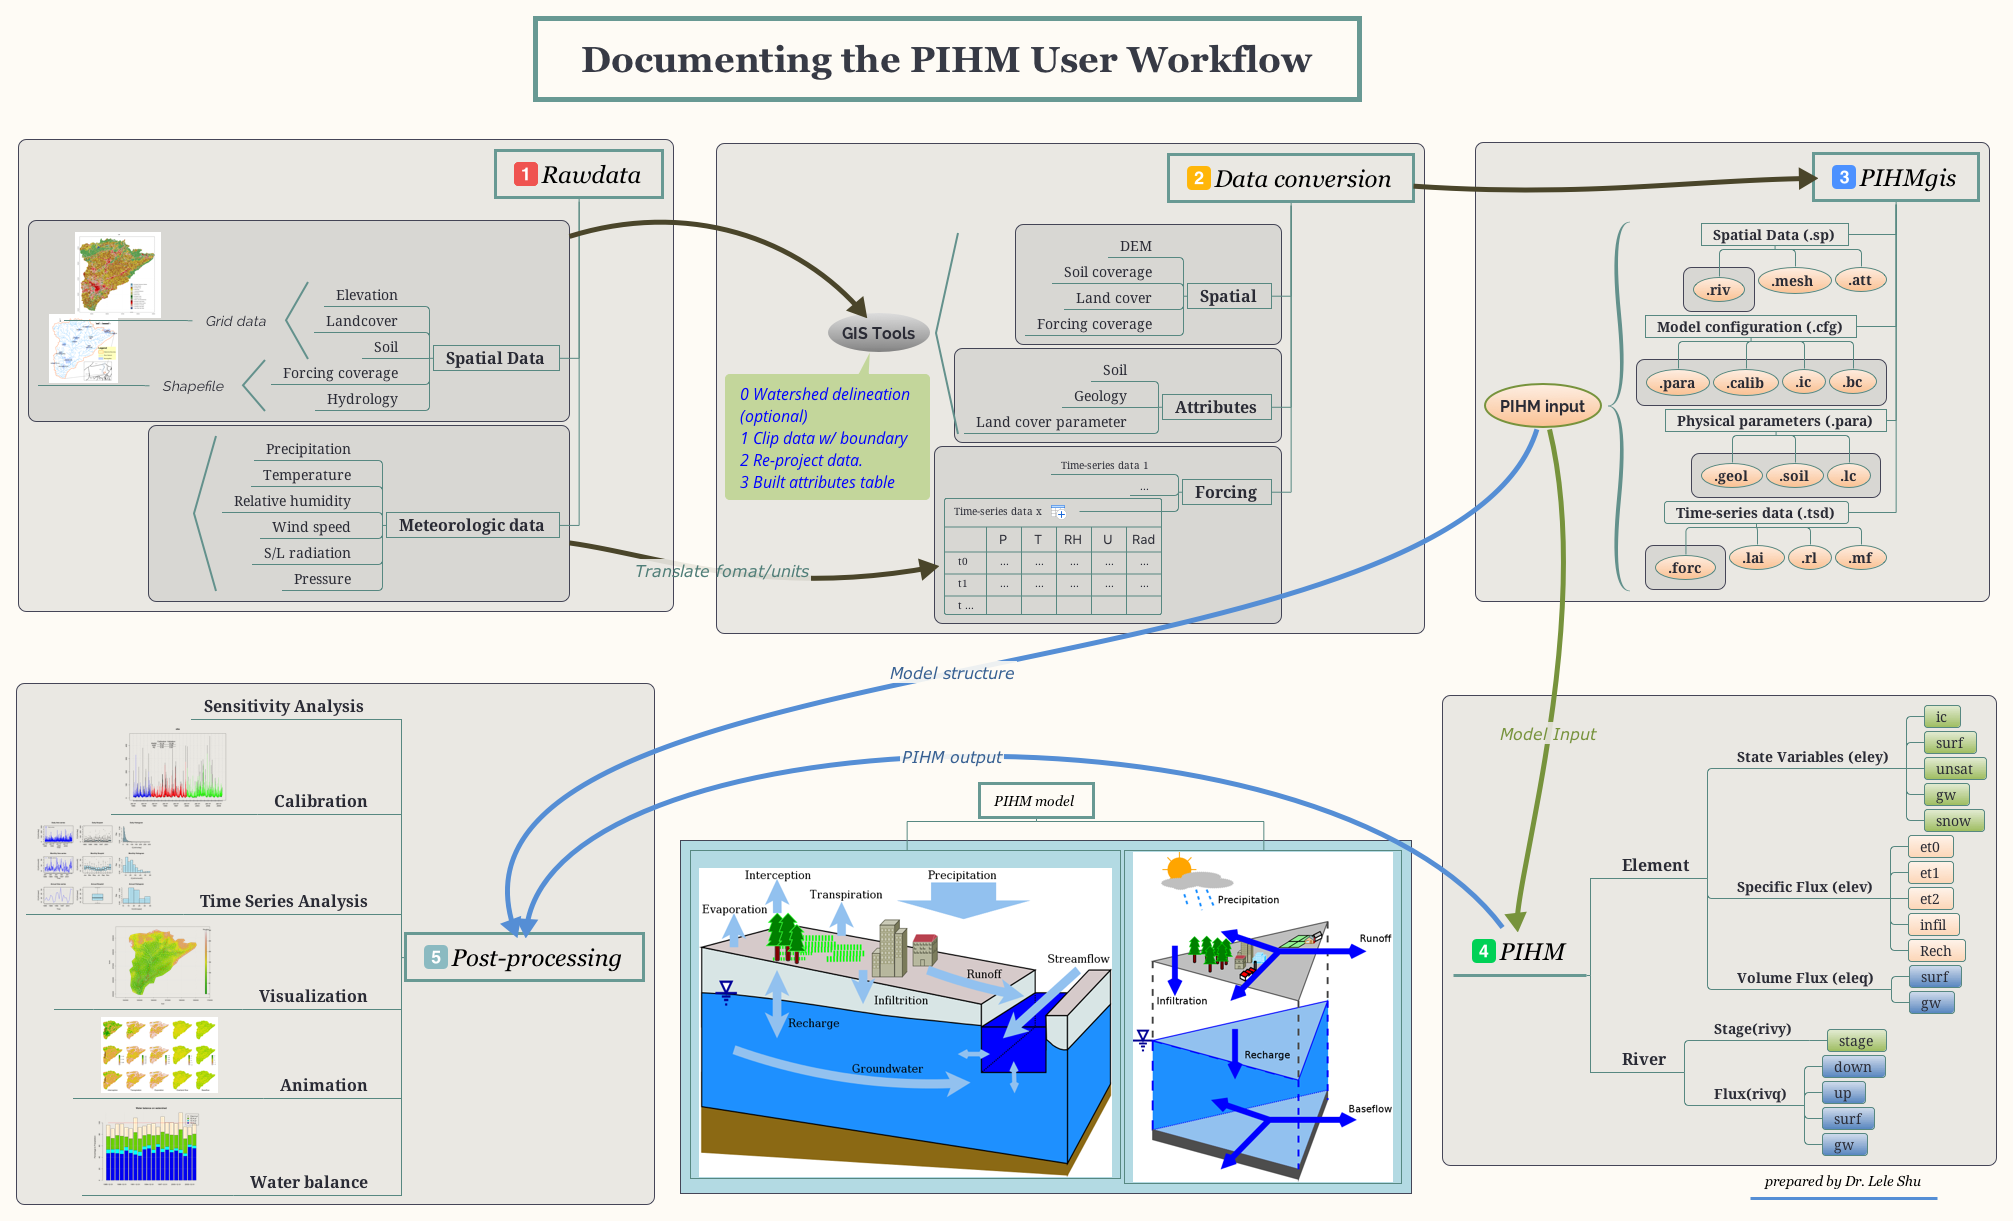
\includegraphics{./Fig/Workflow.png}
\caption{The workflow of modeling with PIHM System}
\end{figure}

\begin{enumerate}
\def\labelenumi{\arabic{enumi}.}
\tightlist
\item
  Prepare raw Essential Terrestrial Variables (ETV)
\item
  Build the PIHM modeling domain with
  \href{http://www.pihm.psu.edu/pihmgis_home.html}{PIHMgis} or
  \href{https://github.com/shulele/PIHMgisR}{PIHMgisR} (Recommended for
  PIHM++)
\item
  Run PIHM on desktop or cluster.
\item
  Analysis the PIHM results with
  \href{https://github.com/shulele/PIHMgisR}{PIHMgisR} or your
  hydrologic analysis tools.
\end{enumerate}

\section{Research with PIHM family}\label{research-with-pihm-family}

\begin{longtable}[]{@{}ccc@{}}
\toprule
Research Ara & Scientific question & Reference\tabularnewline
\midrule
\endhead
Malpasset dam, etc. & Hydrodynamic in dam break and food event &
\citep{Li2011}\tabularnewline
& &\tabularnewline
& &\tabularnewline
& &\tabularnewline
& &\tabularnewline
& &\tabularnewline
& &\tabularnewline
& &\tabularnewline
& &\tabularnewline
\bottomrule
\end{longtable}

\section{Latest update}\label{latest-update}

PIHM++ is the latest version of PIHM, re-developed in C++, a updated
version from the PIHM v2.2 that is the stable and widely applied
version, and that was released on 2010.

The design of PIHM++ is going to advance the PIHM to the new level:

\begin{itemize}
\tightlist
\item
  Technical improvement
\end{itemize}

\begin{enumerate}
\def\labelenumi{\arabic{enumi}.}
\tightlist
\item
  Support the latest implicit Sundial/CVODE solver.
\item
  Re-code the program in object-oriented programming method.
\item
  More human readable input/output files and filenames.
\item
  Support OpenMP and OpenMPI Parrallel computing.
\item
  The functions to handle the time-series data, including forcing, LAI,
  Roughness Length, Boundary Condition, Melt factor.
\item
  Speed up the model performance via coding strategies.
\item
  Screen output the model status and time-spend.
\item
  Fix the bugs in PIHM v2.x.
\end{enumerate}

\begin{itemize}
\tightlist
\item
  Model improvement
\end{itemize}

\begin{enumerate}
\def\labelenumi{\arabic{enumi}.}
\tightlist
\item
  Change the structure/shape of River.
\item
  Add Lakes into the hydrologic process (keep updating).
\item
  CMA-ES calibration, with either OpenMP or OpenMPI.
\item
  Use the Greem-Ampt method to estimate infiltration.
\item
  Add the waterbalance control in elements.
\item
  Hourly update the ET and Potential ET.
\item
  Model debug mode.
\item
  Export model initial condition at specific interval.
\item
  Automatic check the range of physical parameters
\end{enumerate}

\section{Governing equations}\label{governing-equations}

\begin{longtable}[]{@{}llll@{}}
\toprule
\begin{minipage}[b]{0.12\columnwidth}\raggedright\strut
Physical process\strut
\end{minipage} & \begin{minipage}[b]{0.12\columnwidth}\raggedright\strut
Equation name\strut
\end{minipage} & \begin{minipage}[b]{0.31\columnwidth}\raggedright\strut
Governing equation\strut
\end{minipage} & \begin{minipage}[b]{0.31\columnwidth}\raggedright\strut
Semi-discrete formula from ODE\strut
\end{minipage}\tabularnewline
\midrule
\endhead
\begin{minipage}[t]{0.12\columnwidth}\raggedright\strut
Interception\strut
\end{minipage} & \begin{minipage}[t]{0.12\columnwidth}\raggedright\strut
Bucket model\strut
\end{minipage} & \begin{minipage}[t]{0.31\columnwidth}\raggedright\strut
\(\frac{d S_{ic}}{d t} = P - E_{ic}-P_{tf}\)\strut
\end{minipage} & \begin{minipage}[t]{0.31\columnwidth}\raggedright\strut
\(\left(\frac{d S_{ic}}{d t}=R_{veg} * \left(P-E_{I}-P_{t}\right)\right)_{i}\)\strut
\end{minipage}\tabularnewline
\begin{minipage}[t]{0.12\columnwidth}\raggedright\strut
Snow melt\strut
\end{minipage} & \begin{minipage}[t]{0.12\columnwidth}\raggedright\strut
Temperature Index Model\strut
\end{minipage} & \begin{minipage}[t]{0.31\columnwidth}\raggedright\strut
\(\frac{d S_{sn}}{d t}=P-E_{sn}-q_{sm}\)\strut
\end{minipage} & \begin{minipage}[t]{0.31\columnwidth}\raggedright\strut
\(\left(\frac{d S_{sn}}{d t}=P-E_{sn}-q_{sm}\right)_{i}\)\strut
\end{minipage}\tabularnewline
\begin{minipage}[t]{0.12\columnwidth}\raggedright\strut
Overland flow\strut
\end{minipage} & \begin{minipage}[t]{0.12\columnwidth}\raggedright\strut
St.~Venant Equation (2D)\strut
\end{minipage} & \begin{minipage}[t]{0.31\columnwidth}\raggedright\strut
\(\frac{\partial h}{\partial t}+\frac{\partial(u h)}{\partial x}+\frac{\partial(v h)}{\partial y}=q\)\strut
\end{minipage} & \begin{minipage}[t]{0.31\columnwidth}\raggedright\strut
\(\left(\frac{d h}{\partial t} =P_{net}-E_{sf}-q_{inf}-q_{sf}\right)_{i}\)\strut
\end{minipage}\tabularnewline
\begin{minipage}[t]{0.12\columnwidth}\raggedright\strut
Unsaturated zone\strut
\end{minipage} & \begin{minipage}[t]{0.12\columnwidth}\raggedright\strut
Richards Equation\strut
\end{minipage} & \begin{minipage}[t]{0.31\columnwidth}\raggedright\strut
\(C(\psi) \frac{\partial \psi}{\partial t}=\nabla-K(\psi) \cdot \nabla(\psi+Z)\)\strut
\end{minipage} & \begin{minipage}[t]{0.31\columnwidth}\raggedright\strut
\(\left(\frac{d S_{unsat}}{d t}=q_{inf}-q_{rech}-ET_{s}\right)_{i}\)\strut
\end{minipage}\tabularnewline
\begin{minipage}[t]{0.12\columnwidth}\raggedright\strut
Groundwater flow\strut
\end{minipage} & \begin{minipage}[t]{0.12\columnwidth}\raggedright\strut
Richards Equation\$\strut
\end{minipage} & \begin{minipage}[t]{0.31\columnwidth}\raggedright\strut
\(C(\psi) \frac{\partial \psi}{\partial t}=\nabla-K(\psi) \cdot \nabla(\psi+Z)\)\strut
\end{minipage} & \begin{minipage}[t]{0.31\columnwidth}\raggedright\strut
\(\left(S_y \frac{d S}{d t}=q_{rech}+q_{gw}\right)_{i}\)\strut
\end{minipage}\tabularnewline
\begin{minipage}[t]{0.12\columnwidth}\raggedright\strut
River channel\strut
\end{minipage} & \begin{minipage}[t]{0.12\columnwidth}\raggedright\strut
St.~Venant Equation (1D)\strut
\end{minipage} & \begin{minipage}[t]{0.31\columnwidth}\raggedright\strut
\(\frac{\partial h}{\partial t}+\frac{\partial(u h)}{\partial x}=q\)\strut
\end{minipage} & \begin{minipage}[t]{0.31\columnwidth}\raggedright\strut
\(\left(\frac{\partial S}{\partial t} = Q_{up} + Q_{surf} + Q_{sub} + Q_{down} \right)_{i}\)\strut
\end{minipage}\tabularnewline
\bottomrule
\end{longtable}

\chapter{Evapotranspiration}\label{ET}

\section{Hargreaves ETo equation}\label{hargreaves-eto-equation}

\[ {ET}_{{o}}=0.0023\left({T}_{{mean}}+17.8\right)\left({T}_{\max }-{T}_{\min }\right)^{0.5} {R}_{{a}} \]

\section{Penman-Monteith equation}\label{penman-monteith-equation}

The Potential Evapotranspiration (PET) in PIHM++ uses the
Penman-Monteith equation, that combined ``the energy balance with the
mass transfer method and derived an equation to compute the evaporation
from an open water surface from standard climatological records of
sunshine, temperature, humidity and wind speed'' (FAO).

Penman-Monteith Equation is written as:
\[    \lambda ET =  \frac{\Delta (R_n - G) + \rho_a c_p \frac{(e_s -e_a)}{r_a}} {\Delta + \gamma (1+\frac{r_s}{r_a})} \]

\[ \Delta=\frac{4098\left\{0.6108 \exp \left(\frac{17.27 T}{T+237.3}\right)\right]}{(T+237.3)^{2}} \]
\[u_{2}=u_{z_g} \frac{4.87}{\ln (67.8 z_g-5.42)}\]

Bulk surface resistance (\(r_s\)).

\[r_{s}=\frac{r_{l}}{LAI_{\text { active }}}\]

\[LAI_{\text active} = 0.5 LAI\]

Aerodynamic resistance (\(r_a\))
\[r_{a}=\frac{\ln \left[\frac{Z_{m}-d}{Z_{o m}}\right] \ln \left[\frac{Z_{h}-d}{Z_{o h}}\right]}{k^{2} u_{z}}\]
Atmospheric pressure at elevation \(z\) is:
\[P=101.3\left(\frac{293-0.0065 z}{293}\right)^{5.26}\]

\[ \gamma =\frac{C_{p} P}{\varepsilon \lambda}=0.665 \times 10^{-3} P \]

\[RH=100 \frac{{e}_{a}}{e}^{\circ(T)}\]

\[ e^{\circ}(T)=0.6108 \operatorname{exp}\left[ \frac{17.27 T}{{T}+237.3}\right] \]

Where

\begin{itemize}
\tightlist
\item
  \(R_n\) is the net radiation {[}\(J/m^2\){]}
\item
  \(G\) is the soil heat flux {[}\(J/m2\){]},
\item
  \((e_s - e_a)\) represents the vapour pressure deficit of the air
  {[}\(J/m2\){]},
\item
  \(\rho_a\) is the mean air density at constant pressure
  {[}\(kg/m^2\){]}
\item
  \(D\) represents the slope of the saturation vapour pressure
  temperature relationship {[}\(J/m2\){]},
\item
  \(r_s\) and \(r_a\) are the (bulk) surface and aerodynamic resistances
  {[}\(s/m\){]},
\item
  \(LAI\) and \(LAI_{\text active}\) is the Leaf Area Index (LAI) and
  active LAI {[}\(m^2/m^2\){]}.
\item
  \(r_l\) bulk stomatal resistance of the well-illuminated leaf
  {[}\(s/m\){]},
\item
  \(P\) atmospheric pressure {[}\(kPa\){]},
\item
  \(z\) elevation above sea level {[}\(m\){]}
\item
  \(\gamma\) psychrometric constant {[}\(kPa/C\){]},
\item
  \(l\) latent heat of vaporization, 2.45 {[}\(MJ kg-1\){]},
\item
  \(c_p\) specific heat at constant pressure, 1.013*10-3
  {[}\(MJ/kg/°C\){]},
\item
  \(\varepsilon\) ratio molecular weight of water vapour/dry air =
  \(0.622\).
\item
  \(e°(T)\) saturation vapour pressure at the air temperature \(T\)
  {[}\(kPa\){]},
\item
  \(T\) air temperature {[}\(°C\){]},
\item
  \(u_2\) wind speed at 2 m above ground surface {[}\(m/s\){]},
\item
  \(u_{z_g}\) measured wind speed at \(z_g\) \(m\) above ground surface
  {[}\(m/s\){]},
\item
  \(z_g\) height of measurement above ground surface {[}\(m\){]}.
\end{itemize}

\chapter{Landsurface}\label{surf}

Water balance on landsurface of each element.

\[ \frac {dS_{sf}}{dt} = P_{net} - E_{ic} -  q_{inf} - q_{sf} \]

where

\begin{itemize}
\tightlist
\item
  \(S\) Ground water storage {[} \(m\) {]}
\item
  \(q_r\) Recharge to ground water {[} \(m/T\) {]}
\item
  \(q_{sf}\) Horizontal ground water flow at three directions {[}
  \(m^3/T\) {]} \[q_{sf} = \sum_{j=1}^3 {Q_{j} } / {A}\]
\item
  \(Q_{j}\) Horizontal ground water flow at three directions {[}
  \(m^3/T\) {]}
\item
  \(A\) Area of the element, {[} \(m^2\) {]}.
\end{itemize}

\section{Infiltration}\label{infiltration}

Green-Ampt equations.
\[q_{inf} = K_{eff} * \Delta \theta \frac{y0 + h_{f}}{h_f}\]

\begin{Shaded}
\begin{Highlighting}[]
\KeywordTok{library}\NormalTok{(PIHMgisR)}
\NormalTok{y0=}\DecValTok{0}\OperatorTok{:}\DecValTok{100}\OperatorTok{/}\DecValTok{100}
\NormalTok{theta=}\FloatTok{0.5} \OperatorTok{*}\StringTok{ }\NormalTok{(}\DecValTok{0}\OperatorTok{:}\DecValTok{10}\NormalTok{)}\OperatorTok{/}\DecValTok{10}
\NormalTok{Ksat =}\StringTok{ }\FloatTok{0.1} \CommentTok{#m/day}
\NormalTok{qi=theta }\OperatorTok{*}\StringTok{ }\DecValTok{0}
\ControlFlowTok{for}\NormalTok{(i }\ControlFlowTok{in} \DecValTok{1}\OperatorTok{:}\KeywordTok{length}\NormalTok{(theta))\{}
  \ControlFlowTok{for}\NormalTok{(j }\ControlFlowTok{in} \DecValTok{1}\OperatorTok{:}\KeywordTok{length}\NormalTok{(y0))\{}
\NormalTok{    qi[i]=}\KeywordTok{GreenAmpt}\NormalTok{(theta[i], }\DataTypeTok{thetas =} \FloatTok{0.5}\NormalTok{, }\DataTypeTok{ksat =}\NormalTok{ Ksat, }\DataTypeTok{Hfront =} \DecValTok{0}\NormalTok{)}
\NormalTok{  \}}
\NormalTok{\}}
\KeywordTok{plot}\NormalTok{(theta, qi, }\DataTypeTok{ylab=}\StringTok{'Infiltration (m/day)'}\NormalTok{ )}
\end{Highlighting}
\end{Shaded}

\includegraphics{PIHM_Doc_files/figure-latex/unnamed-chunk-2-1.pdf}

\section{Overland flow}\label{overland-flow}

St.~Venant equations Continuity equation

\[ \frac{\partial Q}{\partial x}+\frac{\partial A}{\partial t}=0 \]

Momentum Equation
\[ \frac{1}{A} \frac{\partial Q}{\partial t}+\frac{1}{A} \frac{\partial}{\partial x}\left(\frac{Q^{2}}{A}\right)+g \frac{\partial y}{\partial x}-g\left(S_{o}-S_{f}\right)=0 \]
Assumptions for St.~Venant Equations

\begin{itemize}
\tightlist
\item
  Flow is one-dimensional
\item
  Hydrostatic pressure prevails and vertical accelerations are
  negligible
\item
  Streamline curvature is small.
\item
  Bottom slope of the channel is small.
\item
  Manning's equation is used to describe resistance effects
\item
  The fluid is incompressible
\end{itemize}

\chapter{Unsaturated Zone}\label{unsat}

\[K(\psi)=k_{r}(\psi) K_{s a t}\] Relative pemeability function:
\[k_{r}\left(\Theta_{e}\right)=\Theta_{e}^{1 / 2}\left[1-\left(1-\Theta_{e}^{1 / m}\right)^{m}\right]^{2}\]
Effective saturation as a function of matrix pressure head (van
Genuchten, 1980):

\[\Theta_{e}(\psi)=\frac{\Theta-\Theta_{r}}{1-\Theta_{r}}=\frac{1}{[1+(|\alpha \psi|)^{\beta}] ^ m}  ~~~~~~~~~~ \psi<0\]
\[\Theta_{e}(\psi)={1}  ~~~~~~~~~~ \psi \geq 0\]

Relative permeability is a function of effective saturation
\(\Theta_{e}(\psi)\)(Mualem, 1976)
\[k_{r}\left(\Theta_{e}\right)=\Theta_{e}^{1 / 2}\left[1-\left(1-\Theta_{e}^{1 / m}\right)^{m}\right]^{2}\]

Where - \(\Theta_{r}\)= residual soil moisture {[}dimensionless{]}; -
\(\beta\)= van Genuchten soil parameter, representing the degree of
pore-size uniformity (as \(\beta\) increases, uniformity increases)
{[}dimensionless{]}, (\(m = 1-1/\beta\)) and - \(\alpha\)= van Genuchten
soil parameter, representing the inverse characteristic length of the
soil pores {[}\(1/L\){]}.

\emph{Put a example of the equations, i.e. \(K_e\) along \(\theta\)}

\chapter{Saturated Zone}\label{gw}

\section{Impervious boundary}\label{impervious-boundary}

\section{Horizontal flow}\label{horizontal-flow}

\[ \frac {dS_{gw}}{dt} = q_r + q_{gw}\]

where

\begin{itemize}
\tightlist
\item
  \(S\) Ground water storage {[}\(m\){]}
\item
  \(q_r\) Recharge to ground water {[}\(m/T\){]}
\item
  \(q_{gw}\) Horizontal ground water flow at three directions
  {[}\(m^3/T\){]} \[q_{gw} = \sum_{j=1}^3 Q_{j} / A\]
\item
  \(A\) Area of the elements \(i\), {[}\(m^2\){]}.
\end{itemize}

\chapter{River}\label{Riv}

River water balance: \[
  \frac{d S_{riv}}{d t} = Q_{d} + Q_{s} + Q_{g} + Q_{u}
\] Where:

\begin{itemize}
\tightlist
\item
  \(S_{riv}\) - Water storage in River segments {[}\(m\){]}
\item
  \(Q_{d}\) - Water flux to downstream {[}\(m^3/T\){]}
\item
  \(Q_{s}\) - Surface water flux between river and element
  {[}\(m^/T\){]}
\item
  \(Q_{g}\) - Ground water flux between river and element
  {[}\(m^3/T\){]}
\item
  \(Q_{out}\) - Water flux from upstream(s) {[}\(m^3/T\){]}
\end{itemize}

\[
Q_{d} = \frac{A_{cs}}{n} * {(\frac{A_{cs}}{Y})} ^ {\frac{2}{3}} * \sqrt[]{S} 
\]

where:

\begin{itemize}
\tightlist
\item
  \(A_{cs}\) - Average cross section area of river channels (THIS and
  downstream channel) {[}\(m^2\){]}
\item
  \(n\) - Manning's roughness {[}\(T m^{-\frac{1}{3}}\){]}
\item
  \(Y\) - Mean water level in river channels {[}\(m\){]}
\item
  \(S\) - Slope of river bed {[}\(m/L\){]}
\end{itemize}

\[
Q_s = \frac{2}{3} C_{wr}  L  \sqrt[]{2g} {dH}^ \frac{3}{2}
\] where:

\begin{itemize}
\tightlist
\item
  \$C\_\{wr\} \$ - Weir Discharge Coefficient {[}\(1\){]}
\item
  \(L\) - Length of weir {[}\(m\){]}
\end{itemize}

\chapter{Lake}\label{lake}

Water balance of lake: \[
  \frac{d S_{lake}}{d t} = P - E + ( q_{sf} +  q_{gw} + q_{riv})
\] where

\begin{itemize}
\tightlist
\item
  \(S_{lake}\) Lake water storage {[}\(m\){]}
\item
  \(P\) Precipitation {[}\(m/T\){]}
\item
  \(E\) Evaporation from lake {[}\(m/T\){]}
\item
  \(q_{sf}\) Water flow from landsurface to lake, {[}\(m/T\){]}
  \[q_{sf} = \sum_{j=1}^{Nele} Q_{j}^{sf} / A_{lake}\]
\item
  \(q_{gw}\) Water flow from ground water to lake, {[}\(m/T\){]}
  \[q_{gw} = \sum_{j=1}^{Nele} Q_{j}^{gw} / A_{lake}\]
\item
  \(q_{riv}\) Water PIHM++.pngflow from rivers to lake, {[}\(m/T\){]}
  \[q_{riv} = \sum_{j=1}^{Nriv} Q_{j}^{riv} / A_{lake}\]
\item
  \(Nele\) and \(Nriv\) are number of elements and river adjecent to the
  lake respectively. {[}\(-\){]}
\item
  \(A_i\) Area of the elements \(i\), {[}\(m^2\){]}.
\end{itemize}

\chapter{Calibration}\label{calibration}

The Covriance Matrix Adaptation Evolution Strategy (CMA-ES).

\chapter*{Acknowledge}\label{acknowledge}
\addcontentsline{toc}{chapter}{Acknowledge}

The PIHM Modeling System was initially developed under research grants
to The Pennsylvania State University (Penn State) from NSF (EAR 9876800,
1999-2007; EAR 03-10122, 2003-2007), NOAA (NA040AR4310085, 2003-2007),
NASA (NAG5-12611, 2002-2005), with continuing grants from NSF and EPA
for community model development.

The PIHM model is a continuation of 17 years of modeling in hydrology
and related fields. In addition to the Pennsylvania State University and
Dr.~Christopher Duffy, several guaduate student in Dr.~Duffy group
contributed to the model. We also want to thank all the users in past 17
years who contributed lots of hydrology-related researches that make
PIHM community booming.

Many thanks to contributors in PIHM family:

\begin{longtable}[]{@{}ll@{}}
\toprule
Name & Major Contriution\tabularnewline
\midrule
\endhead
Christopher Duffy & Leader of the PIHM group\tabularnewline
Lele Shu & PIHM++\tabularnewline
& PIHMgisR\tabularnewline
& PIHM analysis tools\tabularnewline
& LUC-PIHM (Land Use Change)\tabularnewline
Yuning Shi & Flux-PIHM\tabularnewline
& MM-PIHM\tabularnewline
Yu Zhang & LE-PIHM (Landscape Evolution)\tabularnewline
& Lake-PIHM\tabularnewline
Chen Bao & RT-PIHM (Reaction transport)\tabularnewline
Xuan Yu & PIHM v2.2\tabularnewline
& BioBGC-PIHM\tabularnewline
Gopal Bhatt & PIHM v2.0;\tabularnewline
& PIHMgis v3.0\tabularnewline
Mukesh Kumar & PIHM v2.0\tabularnewline
Shuangcai Li & PIHM-Sed (Sediment transport)\tabularnewline
Yizhong Qu & PIHM v1.0 --- The first version of PIHM\tabularnewline
\bottomrule
\end{longtable}

\chapter*{License}\label{license}
\addcontentsline{toc}{chapter}{License}

PIHM++ is open source software and the development is coordinated via
the PIHM GitHub page (\href{https://github.com/shulele/PIHM++}{GitHub
Page} ).

Penn State University makes no proprietary claims, either statutory or
otherwise, to this version and release of PIHM and considers PIHM to be
in the public domain for use by any person or entity for any purpose
without any fee or charge.

We request that any PIHM user include a credit to Penn State in any
publications that result from the use of PIHM.

Penn State University makes no proprietary claims, either statutory or
otherwise, to this version and release of PIHM and considers PIHM to be
in the public domain for use by any person or entity for any purpose
without any fee or charge. We request that any PIHM user include a
credit to Penn State in any publications that result from the use of
PIHM.

The names Penn State shall not be used or referenced in any advertising
or publicity which endorses or promotes any products or commercial
entity associated with or using PIHM, or any derivative works thereof,
without the written authorization o Penn State.

PIHM is provided on an ``AS IS'' basis and any warranties, either
express or implied, including but not limited to implied warranties of
noninfringement, originality, merchantability and fitness for a
particular purpose, are disclaimed. Penn State will not be obligated to
provide the user with any support, consulting, training or assistance of
any kind with regard to the use, operation and performance of PIHM nor
to provide the user with any updates, revisions, new versions, error
corrections or ``bug'' fixes. In no event will Penn State be liable for
any damages, whatsoever, whether direct, indirect, consequential or
special, which may result from an action in contract, negligence or
other claim that arises out of or in connection with the access, use or
performance of PIHM, including infringement actions.

\bibliography{book.bib,packages.bib}

\end{document}
